\subsection{Series RLC Underdamped and Critically Damped Behaviour}
\begin{center}
    \begin{circuitikz}
        % Draw a voltage source from 0 to 5V
        \draw (0,0) to [american voltage source, voltage dir=RP, v=$V_{in}$] (0,4);
        \draw (0,4) to [R, l=$100\Omega$] (\linewidth/4,4);
        \draw (\linewidth/4,4) to [L, l=$10\text{mH}$] (\linewidth/2,4);
        % Draw a C that connects to the voltage in
        \draw (\linewidth/2,4) to [C, l=$6\text{n}8\text{F}$] (\linewidth/2,0);
        \draw (\linewidth/2,0) to (0,0);
    \end{circuitikz}
\end{center}

The second order differential equation for this RLC series circuit is solved by remembering that
\begin{equation}
    i = i_C = C\frac{dV_c}{d_t}
\end{equation}
Taking this into account, our mesh will be defined as follows:
\begin{equation}
    V_{in} = V_R + V_C + V_L
\end{equation}
Where each component is defined by their respective relations:
\begin{equation}
    \begin{gathered}
        V_L = L\frac{di}{dt} \\
        V_R = iR \\
        i_C = C\frac{dV_C}{dt}
    \end{gathered}
\end{equation}
Substituting these relations into the mesh equation, the following is obtained:
\begin{equation}
    V_{in} = LC\frac{d^2V_C}{dt^2} + RC\frac{dV_C}{dt} + V_C
\end{equation}
Which is a second-order differential equation. The following constants can now be defined:
\begin{equation}
    a_2 = LC, \quad a_1 = RC, \quad a_0 = 1
\end{equation}
Subsequently, for the proper form of the differential equation the following are defined:
\begin{equation}
    \zeta = \frac{a_1}{2\sqrt{a_0a_2}}, \quad \omega_n = \sqrt{\frac{a_0}{a_2}}
\end{equation}
Using {\bf MATLAB}, the behaviour of the circuit can be verified.
\begin{verbatim}
% For the case where R = 100Ohm, C = 6.8nF and L=10mH
R = 100;
C = 6.8E-9;
L = 10E-3;

zeta = R/2 * sqrt(C/L); % approximately 0.0412, so underdamped
w_n = 1/sqrt(L*C);
w_d = w_n * sqrt(1 - zeta^2);

\end{verbatim}
It is found that
\begin{equation}
    \zeta = 0.0412, \quad \omega_n = 1.2127\times10^5 \text{rad/s} \quad \omega_d = 1.2116\times10^5 \text{rad/s}
\end{equation}
Which indicates that the circuit is underdamped.
The initial conditions can be identified using the total response of the circuit, given by:
\begin{equation}
    y_t(t) = y_h(t) + y_f(t)
\end{equation}

Where $y_h(t)$ is the homogeneous response and $y_f(t)$ is the forced response.

\begin{equation}
    y(t) = e^{-\zeta \omega_n t}\left(C_1\cos(\omega_d t) + C_2\sin(\omega_d t)\right) + V_{in}
\end{equation}

Where $V_{in}$ in this case is simply 1V. At at $t=0$, the voltage over the capacitor is 0V.

\begin{equation}
    y(0) = C_1 + V_{in} \implies y(0) = C_1 + V_{in} \implies C_1 = -V_{in} = -1V.
\end{equation}
Consider that the change over the capacitor is also 0V at immediately $t=0$,
it follows that for:
\begin{equation}
    \frac{dy}{dt} = e^{-\zeta \omega_n t} \left(C_2 \omega_d \cos(\omega_d t) - C_1 \omega_d \sin(\omega_d t)\right) - \omega_n \zeta e^{-\zeta \omega_n t} \left(C_1\cos(\omega_d t) + C_2\sin(\omega_d t)\right)
\end{equation}
Evaluated at $t=0$, it is obtained that:
\begin{equation}
    \begin{gathered}
        \frac{dy}{dt}(0) = C_2 \omega_d - \omega_n \zeta C_1 \\
        0 = C_2 \omega_d - \omega_n \zeta C_1 \\
        C_2 = - \frac{\omega_n}{\omega_d} \zeta
    \end{gathered}
\end{equation}
Which, using {\bf MATLAB}, leads that $C_2 = -0.0413$.
\begin{verbatim}
C1 = -1;
C2 = -(w_n/w_d) * zeta; % -0.0413    
\end{verbatim}

Plotting the data using {\bf MATLAB} the following for the voltage over the capacitor is obtained:

\begin{figure}[H]
    \centering
    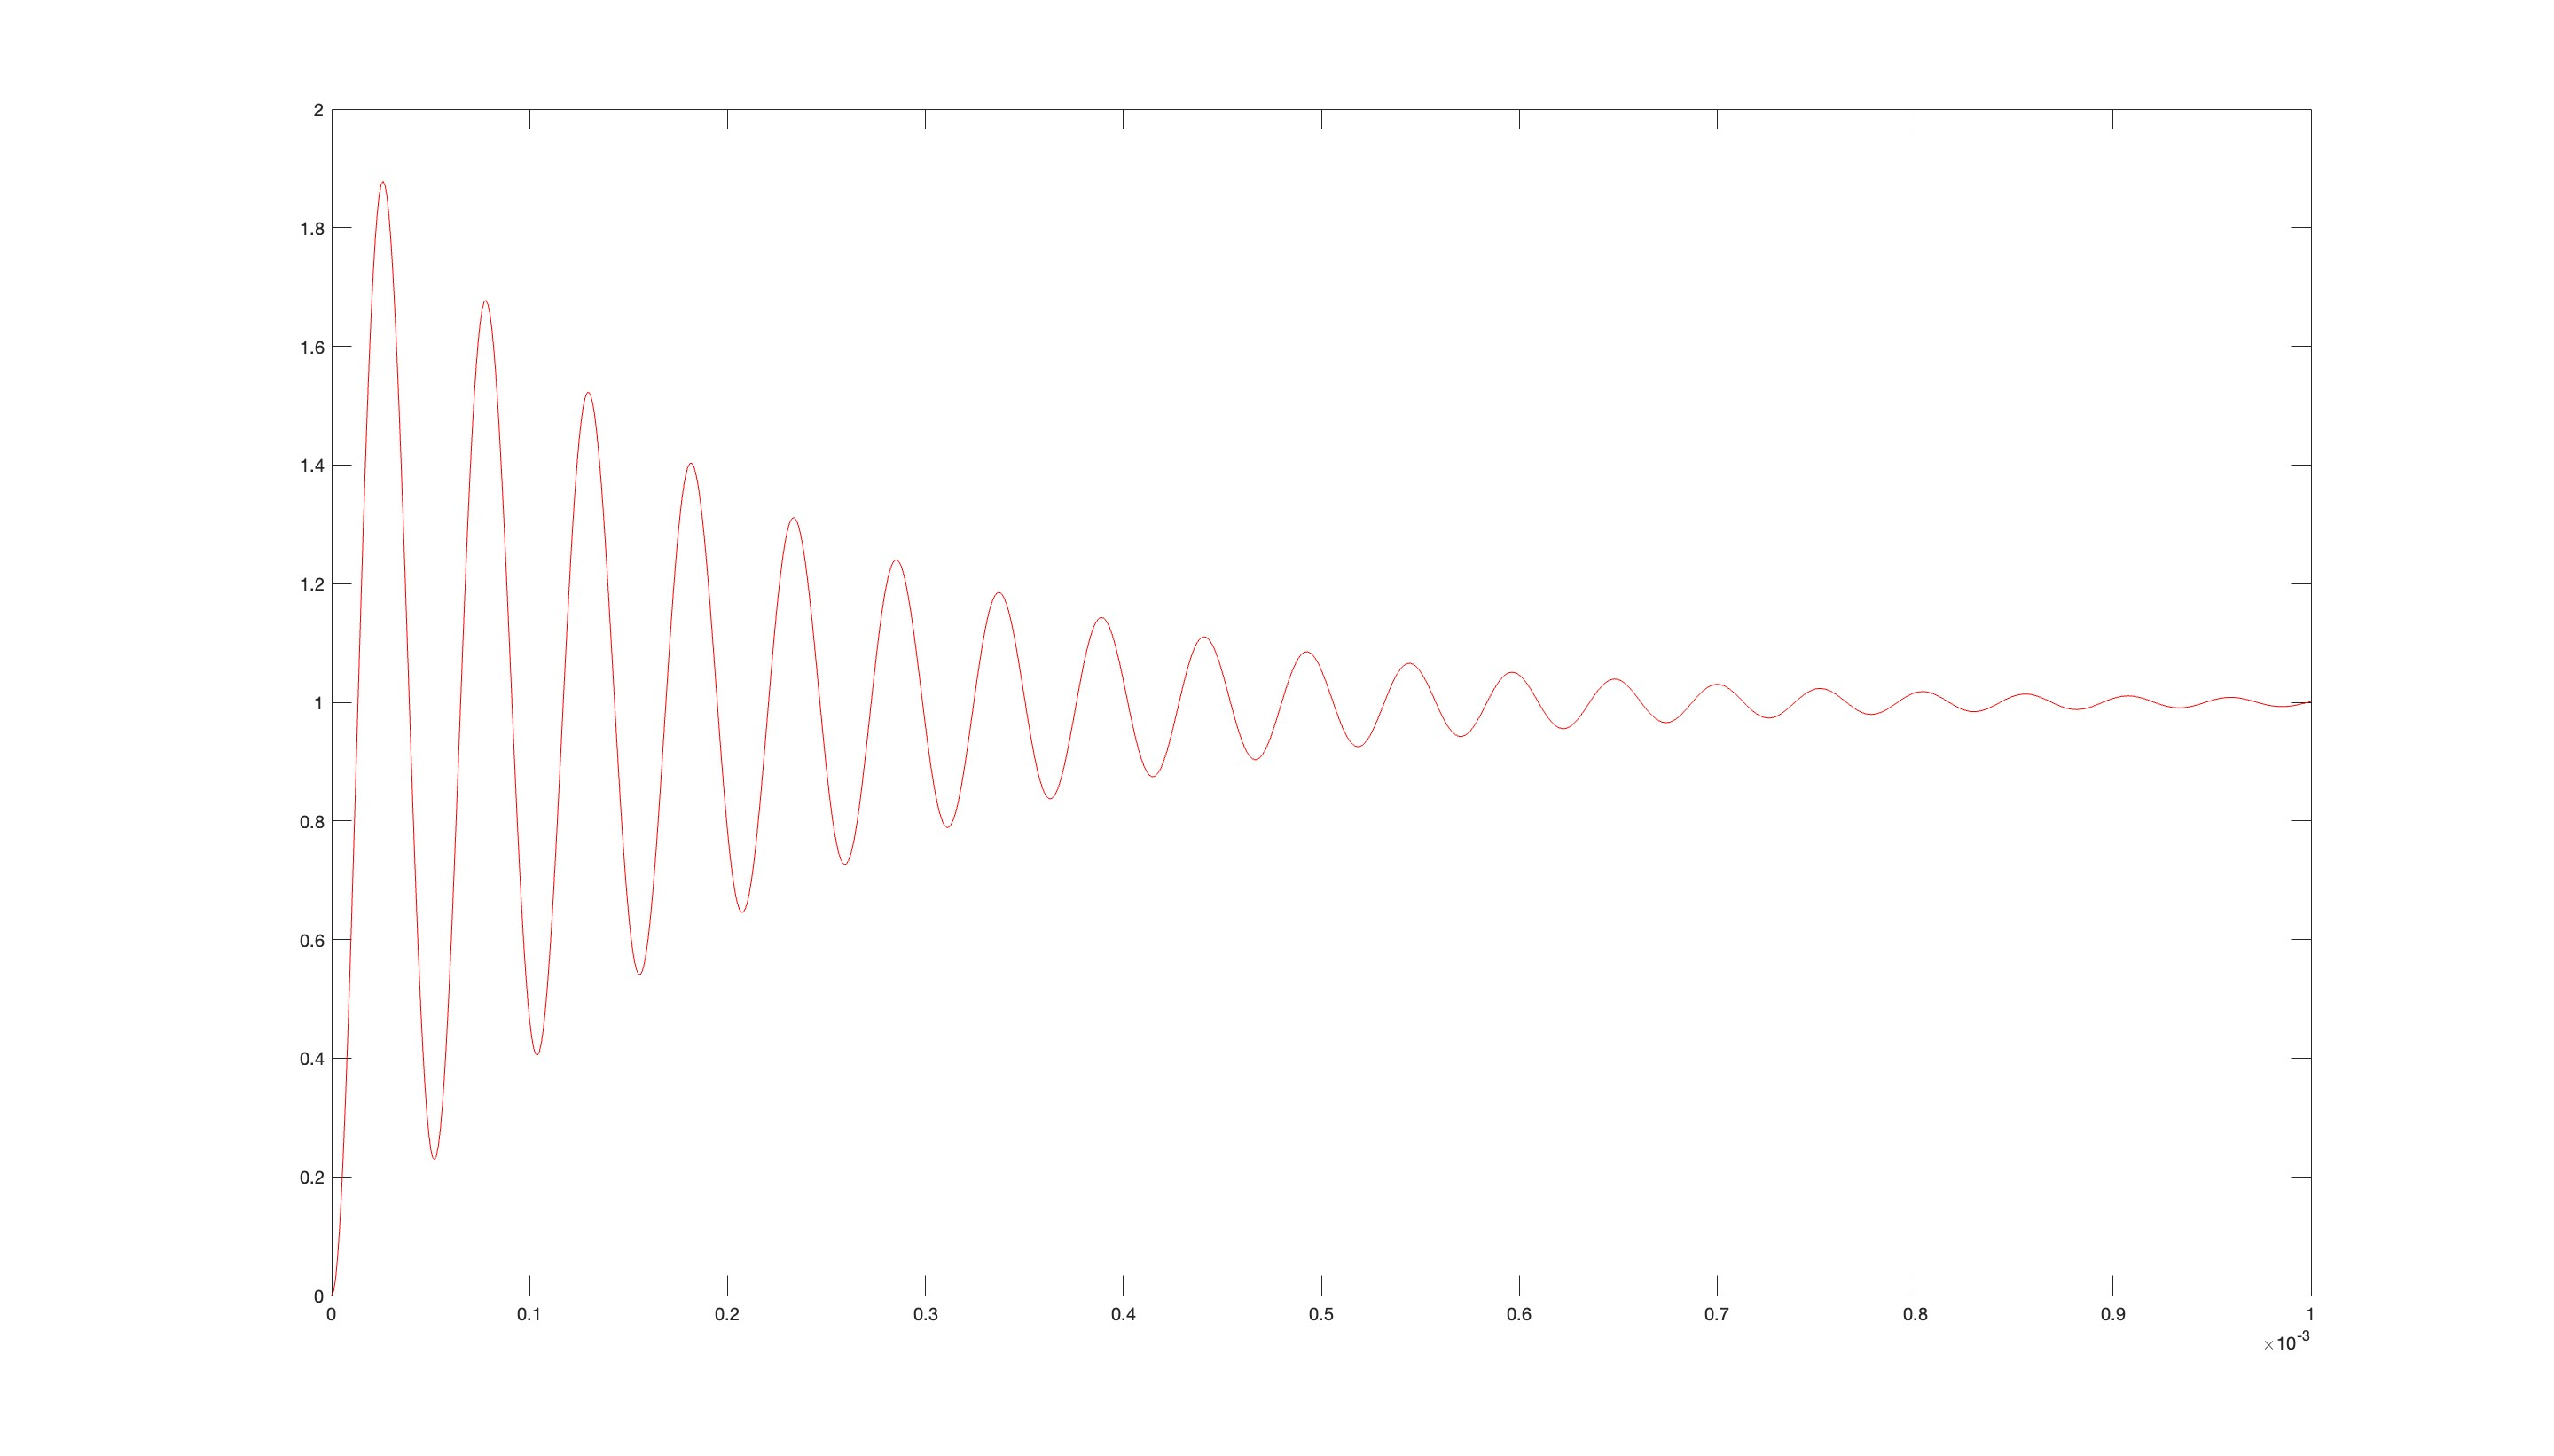
\includegraphics[width=\linewidth]{images/evaluation_vc.jpg}
    \caption{Voltage over the capacitor}
    \label{fig:evaluation_vc}
\end{figure}

Showing that the circuit is indeed underdamped.

In order to get {\bf critically damped} behaviour, $\zeta = 1$. The following relation to find the optimal resistance to make $\zeta$ go to $1$.

\begin{equation}
    \begin{gathered}
        \zeta = \frac{R}{2} \sqrt{C/L} \\
        \text{Knowing that $\zeta = 1$} \\
        R = \frac{2}{\sqrt{C/L}} \\
    \end{gathered}
\end{equation}

For the critically damped circuit, the initial
conditions $C_1$ and $C_2$ can be found by knowing that the general solution
for a critically damped circuit is given

\begin{equation}
    y(t) = e^{-\zeta \omega_n t}\left(C_1 + C_2 t\right) + V_{in}
\end{equation}
Where $V_{in}$ is the particular solution to the differential equation, because at steady state, the voltage over the capacitor is equal to the voltage of the voltage source.

Knowing that $V_{in}$ is 1V, the initial condition $C_1$ straightforwardly can be found:
\begin{equation}
    y(0) = C_1 + V_{in} \implies C_1 = -V_{in} = -1V.
\end{equation}
Finding $C_1$, $C_2$ can be found by taking the derivative
of the general solution for this critically damped circuit:
\begin{equation}
    \frac{dy}{dt} = -\zeta \omega_n C_1 e^{-\zeta \omega_n t} - \zeta w_n C_2 t e^{-\zeta \omega_n t} + C_2 e^{-\zeta \omega_n t}
\end{equation}

Evaluating this at $t=0$, and knowing $\zeta = 1$, it is obtained that:
\begin{equation}
    0 = -\zeta \omega_n C_1 + C_2 \implies C_2 = \zeta \omega_n C_1 \implies C_2 = -\omega_n
\end{equation}

Subsequently, arrive at the conclusion that $C_2 = -1.2127\times10^5$.
Plotting the data using {\bf MATLAB} the following for the voltage over the capacitor in both the critically damped and underdamped cases:

\begin{figure}[H]
    \centering
    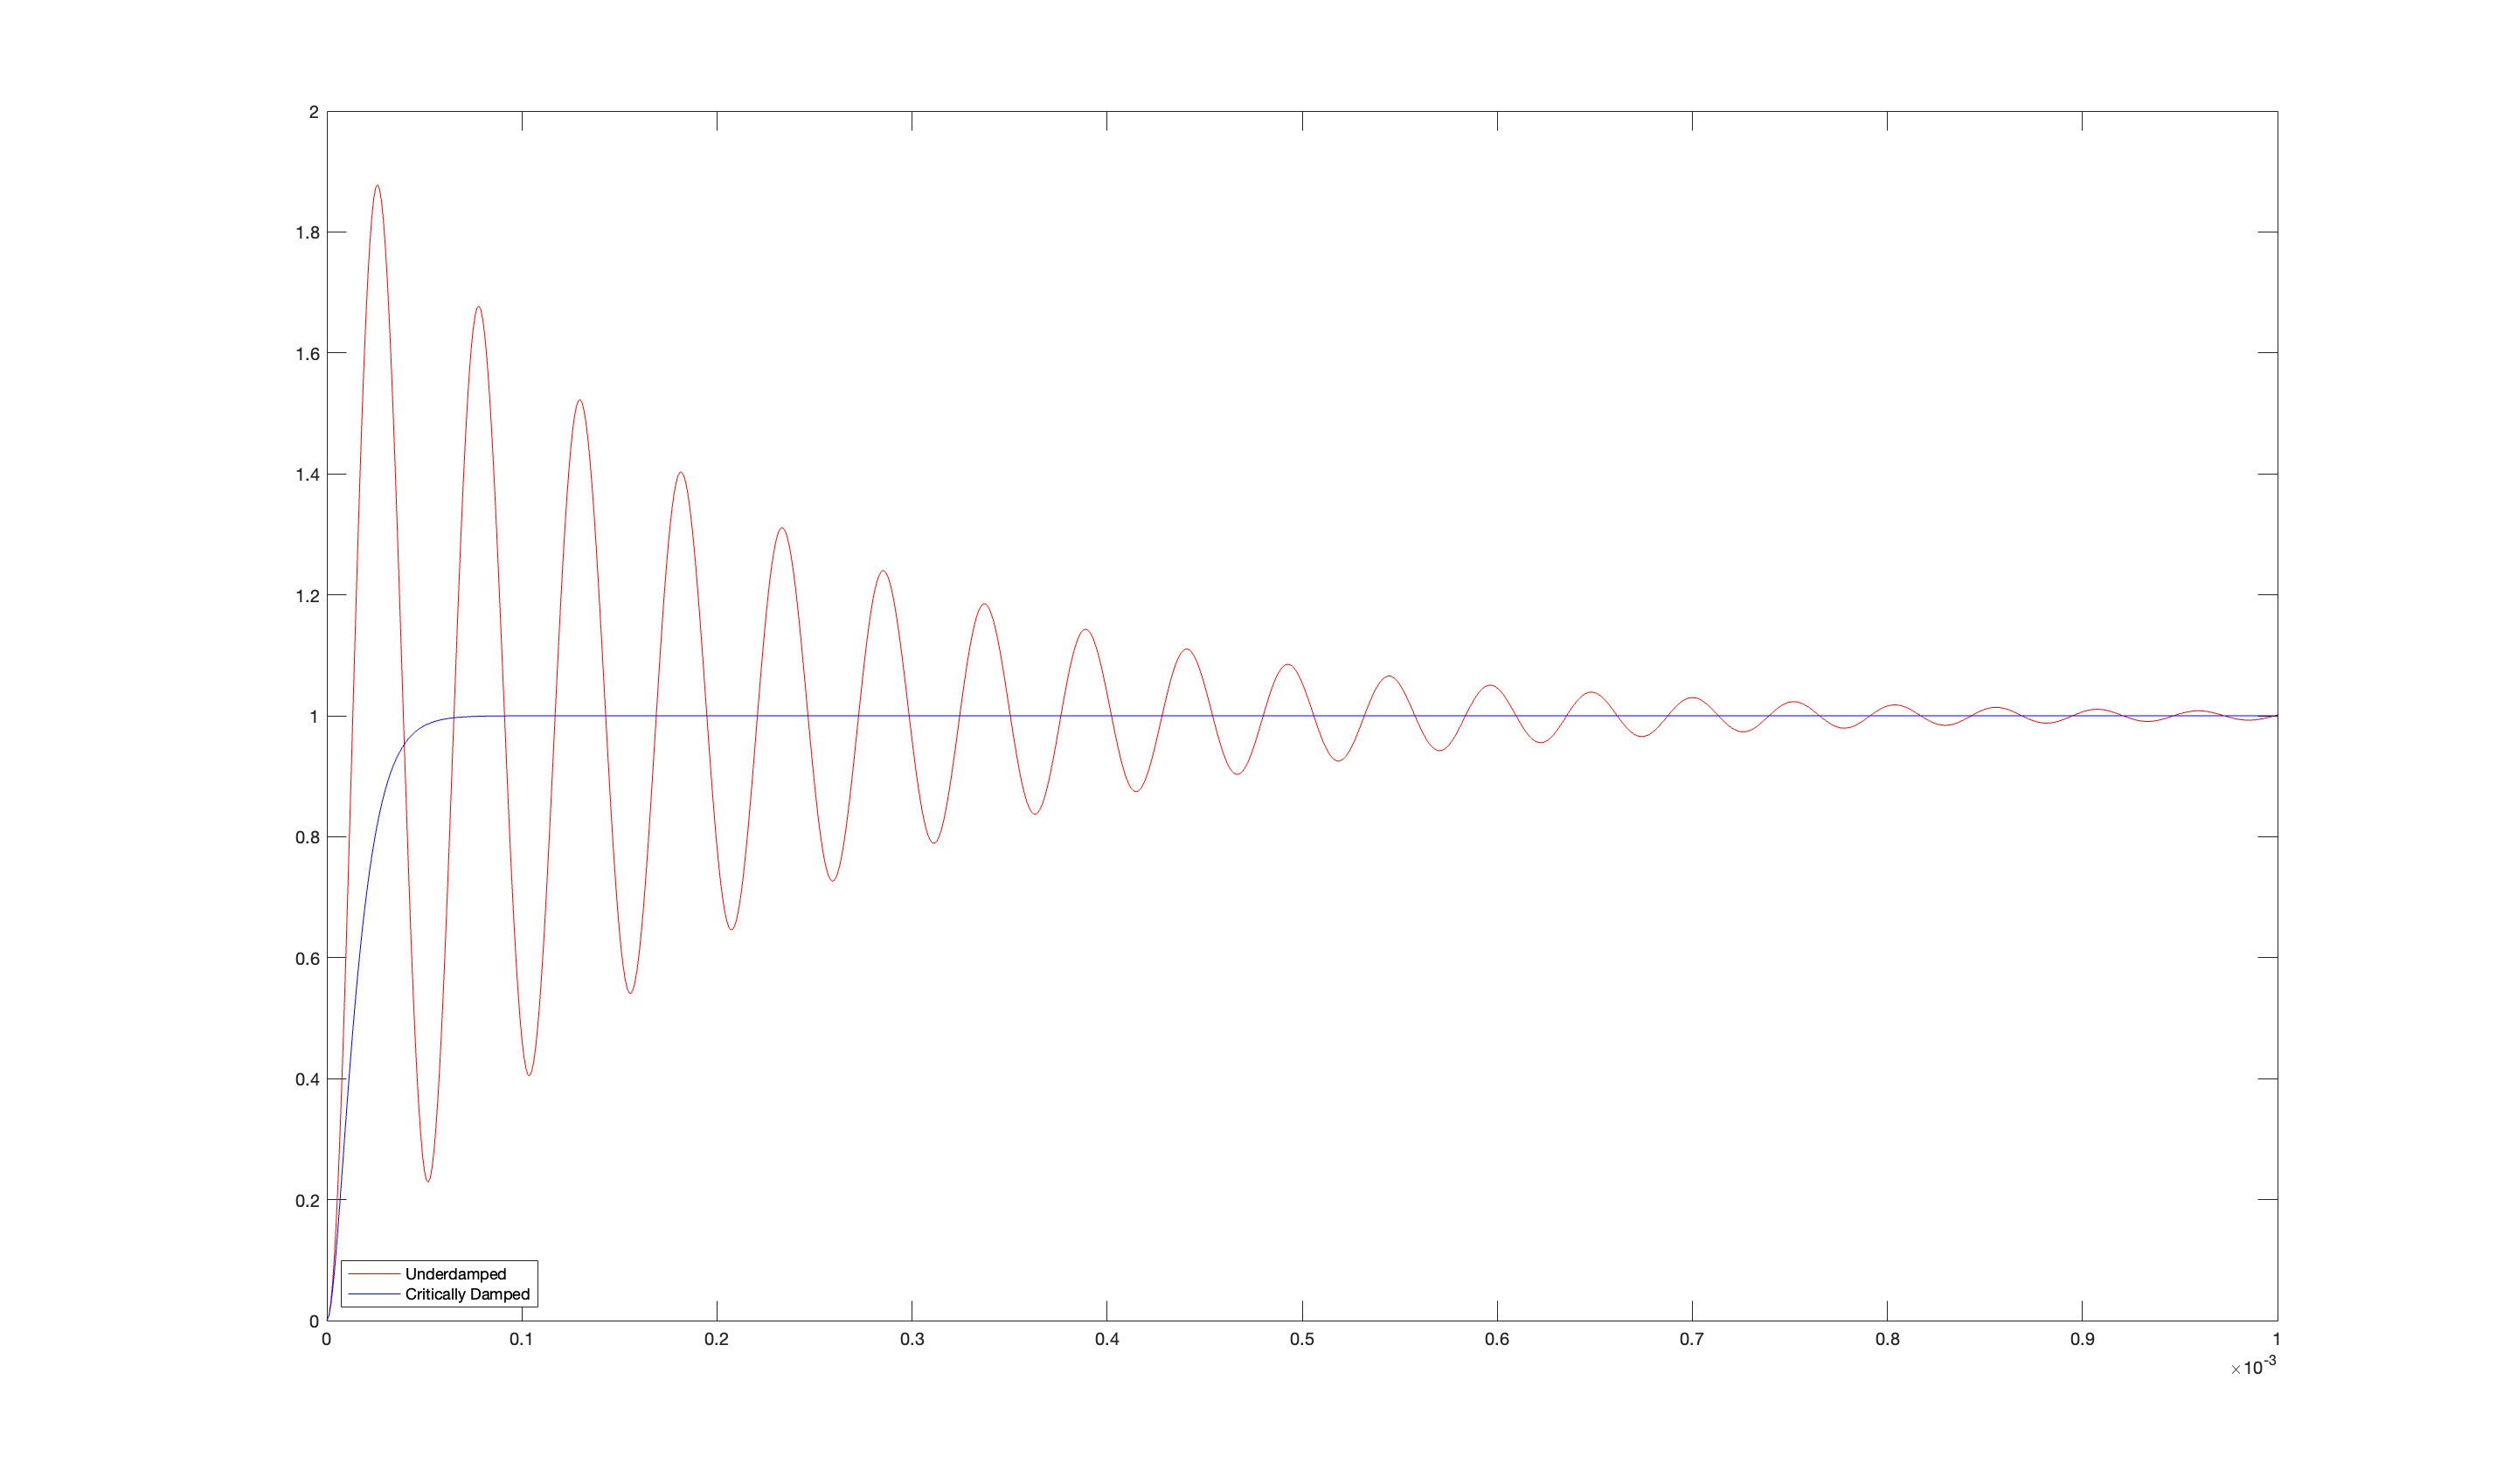
\includegraphics[width=\linewidth]{images/evaluation_vc_full.png}
    \caption{Voltage over the capacitor for both underdamped and critically damped cases}
    \label{fig:evaluation_vc_crit}
\end{figure}

The {\bf MATLAB} code used to generate both of these plots is provided below:
\newpage
\begin{verbatim}
%% Part 1:
clear

% For the case where R = 100Ohm, C = 6.8nF and L=10mH
R = 100;
C = 6.8E-9;
L = 10E-3;

zeta = R/2 * sqrt(C/L); % approximately 0.0412, so underdamped
w_n = 1/sqrt(L*C);
w_d = w_n * sqrt(1 - zeta^2);

% We know that the circuit is underdamped because zeta < 1

% We obtained C1 = -1, C2 = -(w_n/w_d) * zeta
C1 = -1;
C2 = -(w_n/w_d) * zeta;

t = 0:1E-6:1E-3;
y = exp(-zeta * w_n .* t) .* (C1*cos(w_d.*t) + C2 * sin(w_d.*t)) + 1;
plot(t, y, 'red');

hold on

%% Critically damped

% For the critically damped case:
R = 2 * (1 / sqrt(C/L));
zeta = R/2 * sqrt(C/L);
w_n = 1/sqrt(L*C);

% We obtained that C1 = -1, and C2 = -w_n.
C2 = -w_n;
C1 = -1;
y = (C1*exp(-zeta * w_n .* t) + C2.*t.*exp(-zeta * w_n .* t)) + 1;
plot(t, y, 'blue');

legend({'Underdamped','Critically Damped'},'Location','southwest')
\end{verbatim}

Compared to the results obtained in the laboratory, it is observed that the results are very similar, with the only difference being that the voltage over the capacitor in the laboratory when the resistance is at its optimum theoretical value of
$2375\Omega$, where $\zeta$ becomes $1$ and thereby gives us critical damping, gives us a slightly more over-damped response than playing around with the resistance in the R-Decade, which got us a resistance of around $1905\Omega$. This is because of the internal resistance of the R-Decade, which is not taken into account in the theoretical calculations. Furthermore, the theoretical calculations do not take into account the resistance of the wires, the resistance of the capacitor, nor the resistance of the inductor, which all contribute to the overall resistance of the circuit. This is why the theoretical calculations do not match the laboratory results exactly.

\subsection{Circuit Problem}

\begin{figure}[H]
    \centering
    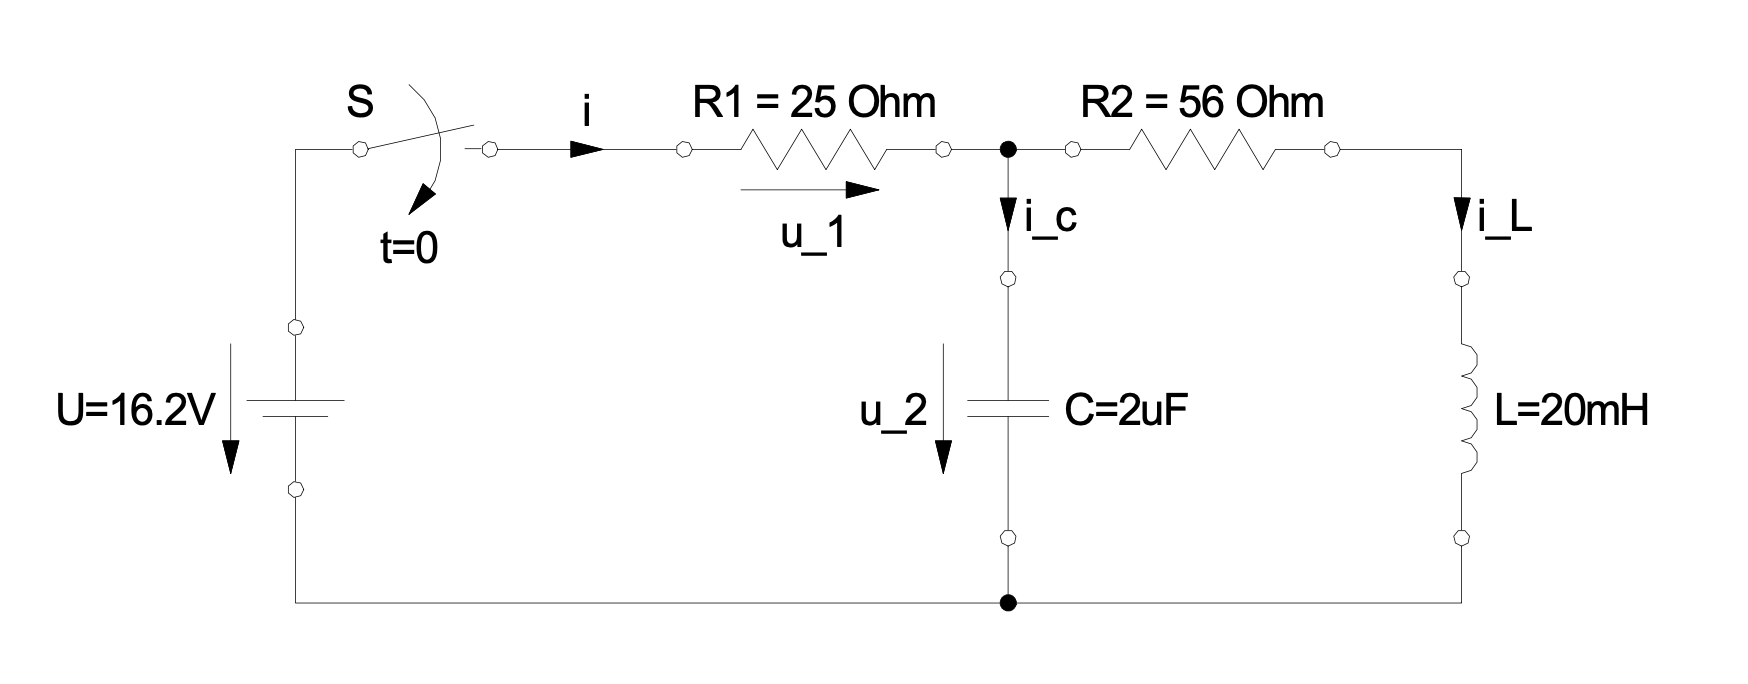
\includegraphics[width=\linewidth]{images/evaluation_circuit.png}
    \caption{The circuit that must be solved.}
    \label{fig:evaluation_circuit}
\end{figure}

To find the current over the inductor $i_L$, first two mesh equations are written:

For the first mesh,
\begin{equation}
    V_{in} = R_1i_1(t) + \frac{1}{C}\int{i_1(t)-i_2(t) dt}
\end{equation}

For the second mesh,
\begin{equation}
    R_2i_2(t)+L\frac{di_2(t)}{dt} + \frac{1}{C}\int{i_2(t)-i_1(t) dt} = 0
\end{equation}

Relations to find $i_2 = i_L$ are obtained. Starting with the second mesh, multiplying both sides by $C$ and by knowing that the integral $\int{i_2(t) - i_1(t)dt}$ can be separated by linearity, it is found that:
\begin{equation}
    \int{i_1(t)dt} = R_2Ci_2(t) + LC\frac{di_2(t)}{dt} + \int{i_2(t)dt}
\end{equation}

Multiplying both sides by $C$ in the first mesh and plugging the found relation, it is found that:

\begin{equation}
    R_1Ci_1 + R_2Ci_2 + LC\frac{di_2(t)}{dt} + \int{i_2(t)dt} - \int{i_2(t) dt} = CV_{in}
\end{equation}

Taking the derivative of equation 3.20, it is obtained:

\begin{equation}
    i_1(t) = R_2C\frac{di_2(t)}{dt}+LC\frac{d^2i_2(t)}{dt^2}+i_2(t)
\end{equation}

This setup allows finding the full differential equation for $i_2 = i_L$.

First, equation 3.21 is divided by C on both sides, and equation 3.22 can be substituted into equation 3.21, which leads to the following:
\begin{equation}
    R_1\left(R_2C\frac{di_2(t)}{dt}+LC\frac{d^2i_2(t)}{dt^2}+i_2(t)\right) + R_2i_2(t) + L\frac{di_2(t)}{dt} = V_{in}
\end{equation}

Normalizing into the standard form of a second order differential equation, the following is obtained:

\begin{equation}
    (R_1LC)\frac{d^2i_2(t)}{dt^2} + (R_1R_2C+L)\frac{di_2(t)}{dt} + (R_1+R_2)i_2(t) = V_{in}
\end{equation}

Where the following constants can now be denoted:
\begin{equation}
    a_2 = R_1LC, \quad a_1 = R_1R_2C+L, \quad a_0 = R_1+R_2
\end{equation}

This information can be used to find the damping ratio of the circuit $\zeta$, which can be used to find the behaviour of the circuit.
By {\bf MATLAB}, it is found that $\zeta = 1.266$, which means the circuit is {\bf overdamped}. Furthermore, it is found that $\omega_n = 9000\text{rad/s}$

The {\bf MATLAB} code used to find the damping ratio, gain, and the natural frequency is provided below:

\begin{verbatim}
R1 = 25;
R2 = 56;
L = 20E-3;
C = 2E-6;
Vin = 16.2;

a2 = R1*L*C;
a1 = R1*R2*C + L;
a0 = R1+R2;

w_n = sqrt(a0 / a2);
zeta = a1 / (2*sqrt(a0 * a2));
K = 1/a0;
\end{verbatim}

The complete response of the circuit is given by:
\begin{equation}
    y(t) = C_1e^{\left(-\zeta + \sqrt{\zeta^2 - 1}\right)\omega_n t} + C_2e^{\left(-\zeta - \sqrt{\zeta^2 - 1}\right)\omega_n t} + i_{Lp}(t)
\end{equation}

Where $i_{Lp}$ is the particular solution to the differential equation, which is given by:

\begin{equation}
    i_{Lp} = \frac{V_{in}}{R_1+R_2} = 0.2\text{A}
\end{equation}

Because the inductor at the steady state becomes a wire.
It must also be noted that for $t=0$:
\begin{equation}
    i_L(0) = 0, \quad \frac{di_L}{dt}(0) = 0
\end{equation}

Because in the transient state, the inductor is an open-circuit to sudden changes of current.

Solving for the initial conditions:
\begin{equation}
    \begin{gathered}
        y(0) = C_1 + C_2 + i_{Lp} \\
        0 = C_1 + C_2 + i_{Lp} \\
        C_1 = -C_2 - i_{Lp}
    \end{gathered}
\end{equation}

Solving for $C_2$:
\begin{equation}
    \begin{gathered}
        \frac{di_L}{dt}(0) = \frac{d}{dt}(C_1e^{\left(-\zeta + \sqrt{\zeta^2 - 1}\right)\omega_n t} + C_2e^{\left(-\zeta - \sqrt{\zeta^2 - 1}\right)\omega_n t} + i_{Lp}(t)) \\
        0 = ((-\zeta + \sqrt{\zeta^2 - 1})\omega_n)C_1e^{\left(-\zeta + \sqrt{\zeta^2 - 1}\right)\omega_n t} + ((-\zeta - \sqrt{\zeta^2 - 1})\omega_n)C_2e^{(-\zeta - \sqrt{\zeta^2 - 1})\omega_n t} \\
        0 = \omega_n\left((-\zeta + \sqrt{-\zeta^2 - 1})(-C_2 - i_{Lp}) + (-\zeta - \sqrt{-\zeta^2 - 1})C_2\right) \\
        0 = -2C_2\sqrt{\zeta^2 - 1} + \zeta i_{Lp} - i_{Lp} \sqrt{\zeta^2 -1} \\
        C_2 = \frac{i_{Lp}(\zeta - \sqrt{\zeta^2 - 1})}{2\sqrt{\zeta^2 - 1}} \\
        C_2 = 0.0629 \\
        C_1 = -C_2 - i_{Lp} = -0.2629
    \end{gathered}
\end{equation}

\begin{figure}[H]
    \centering
    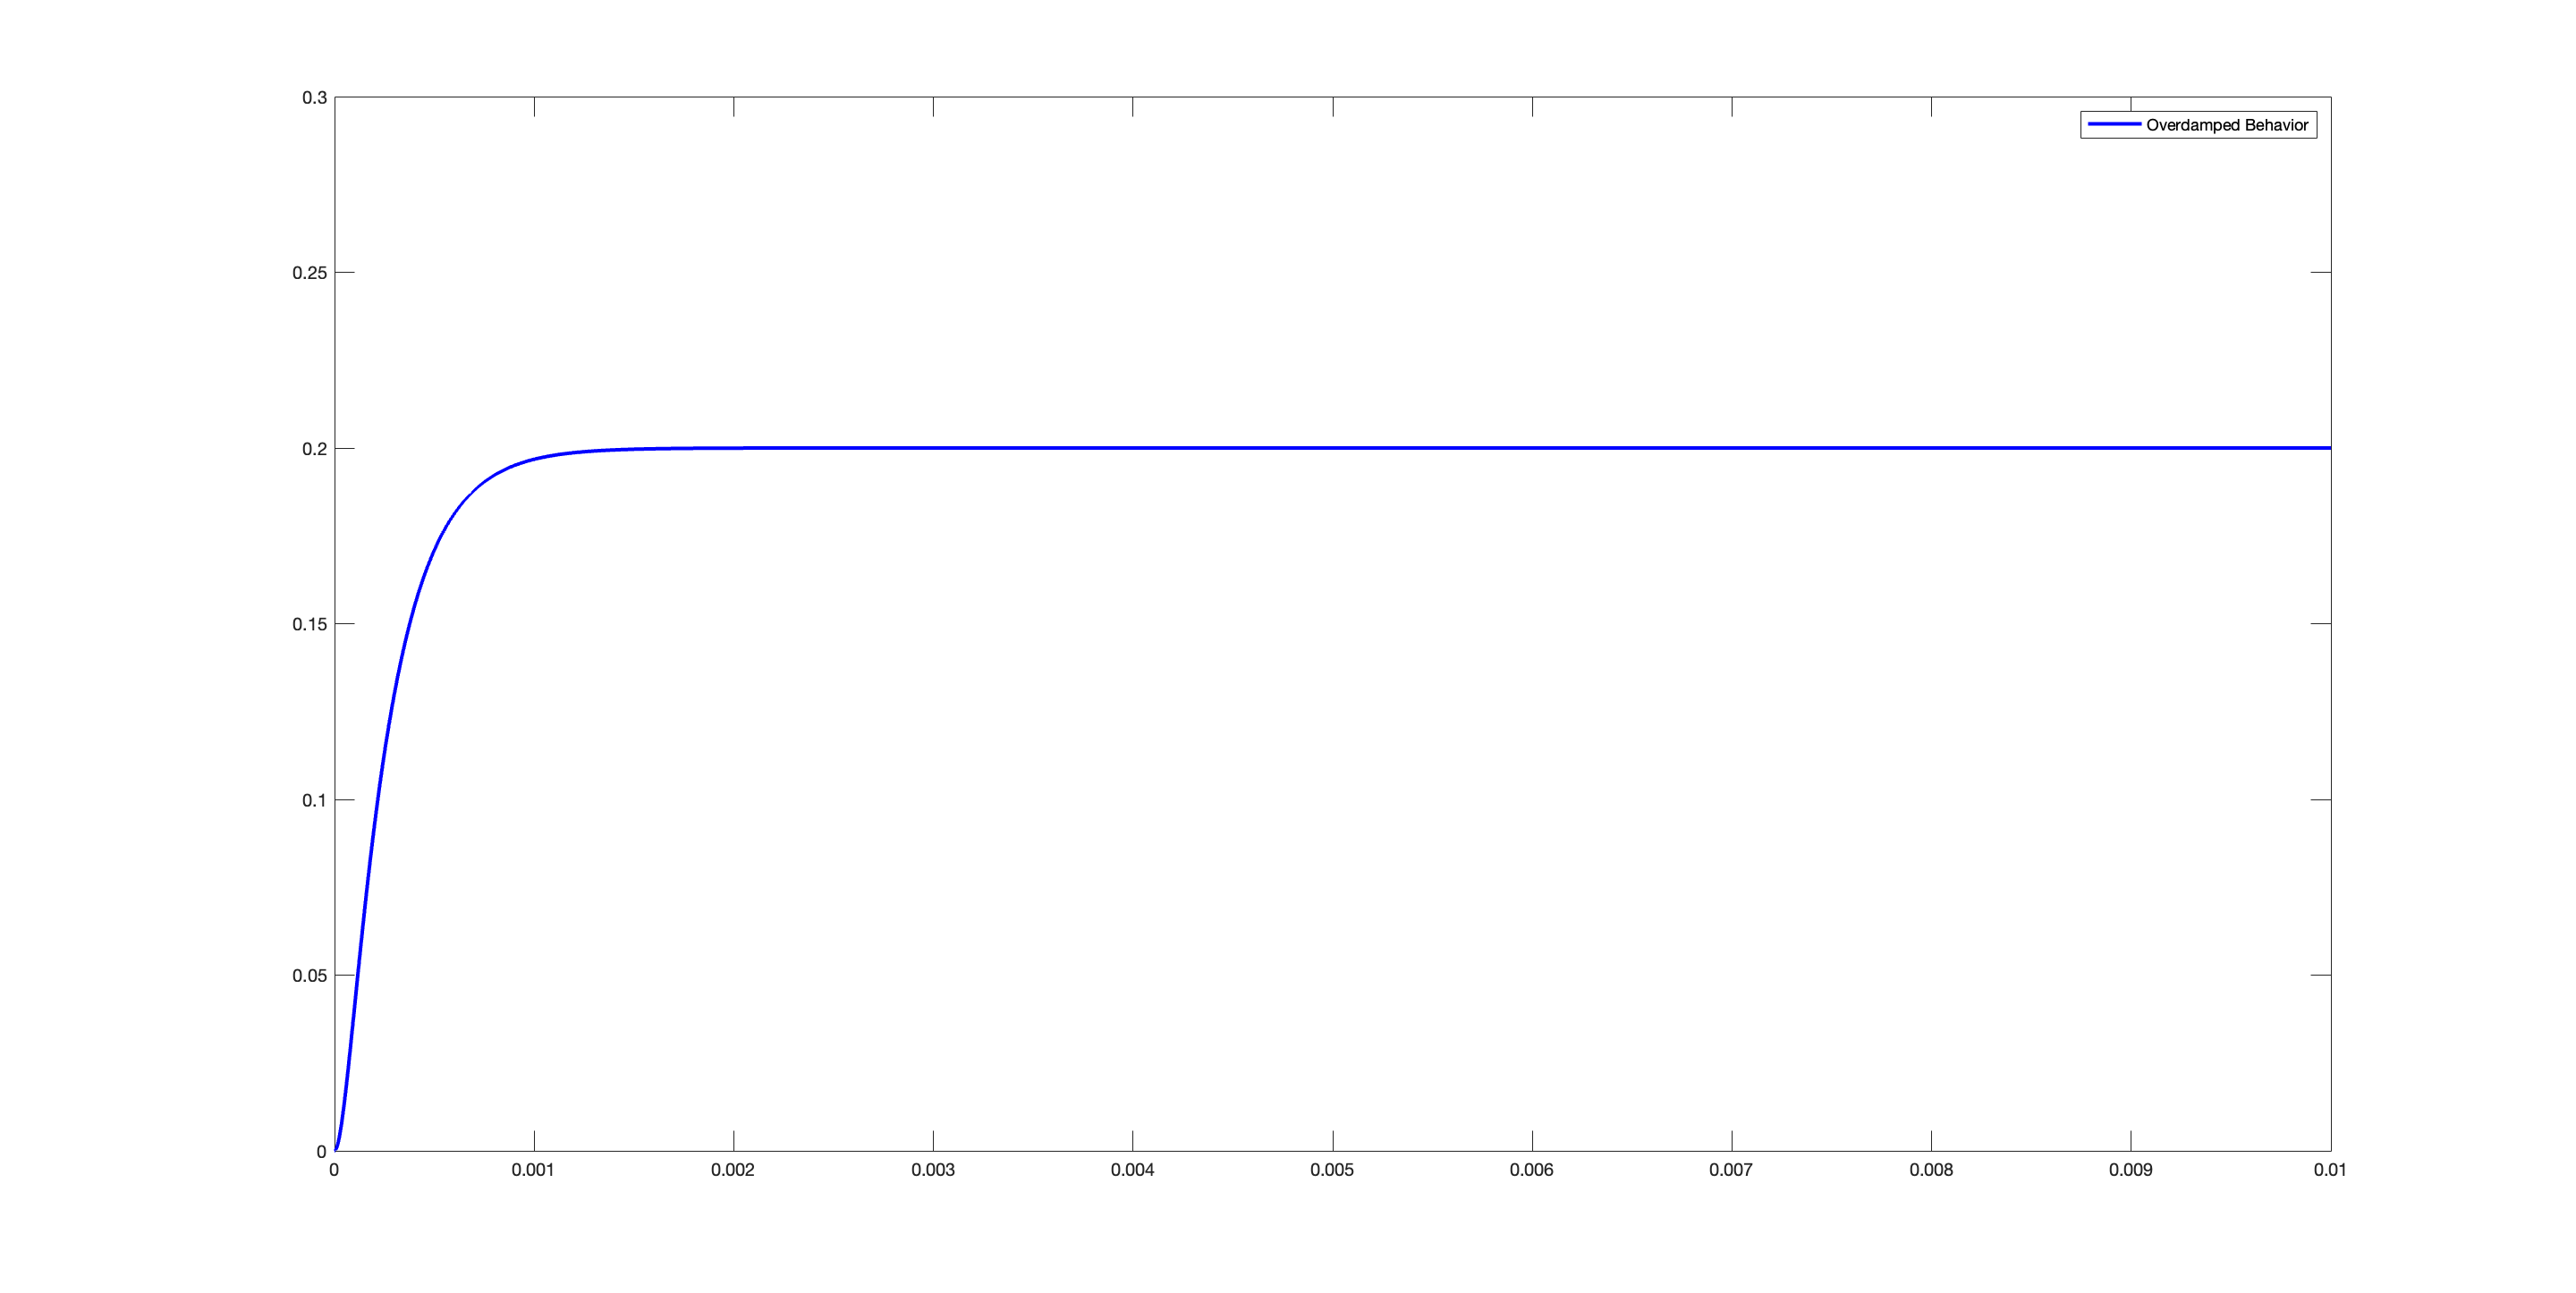
\includegraphics[width=\linewidth]{images/evaluation_iL.png}
    \caption{The current over the inductor.}
    \label{fig:evaluation_iL}
\end{figure}

Using $C_1, C_2 \text{ and } i_{Lp}$, the full response of the circuit is plotted using {\bf MATLAB} with the code provided below.
\newpage
\begin{verbatim}
R1 = 25;
R2 = 56;
L = 20E-3;
C = 2E-6;
Vin = 16.2;

a2 = R1*L*C;
a1 = R1*R2*C + L;
a0 = R1+R2;

w_n = sqrt(a0 / a2);
zeta = a1 / (2*sqrt(a0 * a2));
K = 1/a0;

iL_p = Vin / (R1 + R2);
C2 = iL_p * (zeta - sqrt(zeta^2 - 1)) / (2 * sqrt(zeta^2 - 1));
C1 = -C2 - iL_p;

% The current over the inductor.
t = 0:1E-6:1E-2;
% It is overdamped.
y = C1 .* exp((-zeta + sqrt(zeta^2 - 1)) .* t .* w_n) + ...
        C2 .* exp((-zeta - sqrt(zeta^2 - 1)) .* t .* w_n) + iL_p;

plot(t, y, "blue", "LineWidth", 2);
ylim([0, 0.3])
legend("Overdamped Behavior")
\end{verbatim}